\documentclass[11pt,a4paper]{article}
\usepackage[utf8]{inputenc}
\usepackage[T1]{fontenc}
\usepackage[polish]{babel}
\usepackage{lmodern}
\usepackage{graphicx}
\usepackage{epstopdf}
\usepackage{anysize}
\usepackage{makeidx}
\usepackage{hyperref}



\makeatletter
\renewcommand{\maketitle}{
\begin{titlepage}
\begin{center}

\LARGE{AKADEMIA GÓRNICZO-HUTNICZA}

\vspace*{1cm}

\includegraphics[scale=1.8]{agh.eps}
\vspace*{1cm}

\LARGE{im. Stanisława Staszica w Krakowie}

\rule{\textwidth}{0.4mm}
\LARGE \textsc{\@title}
\rule{\textwidth}{0.4mm}

\vspace*{5mm}


\large
\emph{Autorzy:}\\
Bartłomiej \textsc{Bułat}\\
Tomasz \textsc{Czarnik}\\
Krzysztof \textsc{Śmiłek}\\

\vfill
\vspace*{\stretch{8}}
\rule{\textwidth}{0.4mm}

\large{Wydział Elektroniki, Automatyki, Informatyki i Elektrotechniki}\\
\large{Katedra Automatyki}\\
\large{Laboratorium Biocybernetyki}\\
\vspace*{\stretch{7}}
\@date

\end{center}

\end{titlepage}
}
\makeatother

\title{Metody rozpoznawania twarzy \\przegląd i porównanie}
\date{\today}

\makeindex

\begin{document}

\maketitle

\newpage

\tableofcontents

\newpage

\section{Wstęp}

Rozpoznawanie twarzy od zawsze było dla ludzi najbardziej naturalnym sposobem identyfikacji osób. Małe dzieci bez trudu rozpoznają twarze swoich rodziców. Nie sprawia nam również większego problemu odnajdywanie twarzy nawet na bardzo złożonych obrazach. Potrafimy też określić płeć, przybliżony wiek i pochodzenie tylko na podstawie zdjęcia twarzy danej osoby. Nie dziwi więc fakt, że w dobie prężnie rozwijającej się technologii, coraz szybszych komputerów i ogólnego postępu szukamy sposobów na w pełni automatyczne, cyfrowe metody odnajdywania oraz rozpoznawania twarzy. Zastosowań takich rozwiązań nie trzeba długo szukać: począwszy od rozrywki (konsole nowej generacji, rozpoznawanie osób i uśmiechu w aparatach fotograficznych) przez metody autoryzacji (logowanie na komputerze, w banku) a skończywszy na bezpieczeństwie kraju (rozpoznawanie terrorystów na lotnisku).  Zagadnienie to nie jest nowe, powstało już wiele mniej lub bardziej skutecznych algorytmów. Celem niniejszej pracy jest przegląd popularniejszych rozwiązań i próba ich porównania.

\subsection{Problem rozpoznawania twarzy i ogólny algorytm}

Rozpoznanie twarzy na obrazie nie jest trywialnym problemem. Składa się ono z kilku etapów o różnej złożoności.

Pierwszym etapem jest akwizycja obrazu. Zadanie to jest o tyle trudne o ile trudno jest otrzymać dobry obraz twarzy \emph{en face} na jednolitym tle. W systemach monitoringu taka sytuacja jest prawie niemożliwa. Dlatego dodatkowym zadaniem jest preprocesing obrazu mający na celu uwydatnienie cech charakterystycznych ułatwiających lokalizację. Oprócz tradycyjnej akwizycji kolorowego obrazu 2D wykorzystywane są zdjęcia termowizyjne, które dostarczają  informacji o rozkładzie temperatur oraz obrazy 3D uzyskane metodą stereowizji lub ze specjalnych skanerów.

Kolejnym etapem po akwizycji i preprocesingu jest lokalizacja obiektów które pasują do opisu podstawowych cech twarzy jak kolor czy kształt. Zlokalizowane obiekty są następnie opisywane wektorem cech i klasyfikowane metodami statystycznymi lub przy użyciu sieci neuronowych. Ekstrakcja cech odbywa się za pomocą metod strukturalnych bazujących na cechach lokalnych twarzy oraz metody całościowe, np. PCA.

\subsection{Podział metod}

Metody rozpoznawania twarzy można podzielić na cztery kategorie\cite{YANG001}:

\subsubsection{Metody oparte na wiedzy}

Metoda bazująca na ludzkiej wiedzy tym z jakich elementów i jaki relacji między tymi elementami składa się twarz. Metody te są stosowane głownie do lokalizacji twarzy.

W tym podejściu rozpoznanie twarzy polega na definicji reguł wyprowadzony ze studiów na b   udową ludzkiej twarzy. Można założyć, że twarz na obrazie zwykle pojawia się z dwojgiem oczu, nosem i ustami. Relacjami między tymi elementami może być względna odległość lub położenie.

Trudnością w tym podejściu jest przełożenie wiedzy na dobrze zdefiniowane reguły. Jeśli reguły są zbyt ścisłe, zostaje odrzuconych zbyt wiele prawdziwych twarzy, znowu, gdy reguły są zbyt ogólne dostajemy zbyt wiele fałszywych dopasowań.

\subsubsection{Podejście oparte o cechy stałe}

Podejście to ma na celu wyszukiwanie cech które nie są zależne od oświetlenia czy ułożenia twarzy. Cechy takie jak brwi, oczy, nos, usta czy linia włosów są dobrze wykrywane przez filtry gradientowe. Inną cechą niezmienniczą może być również kolor skóry, który daje się łatwo wyekstrahować w odpowiedniej przestrzeni kolorów. Bazując na uzyskanych cechach budowany jest ich model statystyczny do określenia zależności miedzy cechami i do weryfikacji istnienia twarzy.

\subsubsection{Metody dopasowania wzorców}

W metodach dopasowywania wzorców standardowy szablon jest ręcznie zdefiniowany i parametryzowany przez funkcję. Z obrazem wejściowym liczona jest korelacja miedzy standardowym szablonem i to ona determinuje istnienie twarzy na obrazie. Zaletą tych rozwiązań jest prostota implementacji. Rozszerzeniem metody są deformowalne szablony mogące dopasować się do pozycji, skali i kształtu znalezionej twarzy.

\subsubsection{Metody oparte o wygląd}

W przeciwieństwie do metody dopasowania wzorców szablony są "wyuczone" z przykładowych obrazów. Ogólnie metody te działają w oparciu o techniki analizy statycznej i uczenia maszynowego w calu znalezienia charakterystyki dla obrazów z twarzą i bez. Wyuczona charakterystyka reprezentowana jest jako model rozkładu prawdopodobieństwa lub funkcji dyskryminacyjnej. Redukcja wymiarów modelu jest zależna od potrzebnej wydajności obliczeń i jej jakości.

\section{Metody Rozpoznawania Twarzy}

\subsection{Metody geometryczne}
W metodach tych twarz charakteryzowana jest przez zbiór wartości kątów, odległości czy też pól wyznaczonych w oparciu o charakterystyczne punkty, takie jak środki oczu, koniec nosa itd. Problemem jest tutaj precyzyjne zlokalizowanie odpowiednich fragmentów twarzy. Staje się to szczególnie trudne gdy zdjęcie poddane analizie nie jest wykonane bezpośrednio od przodu, gdyż wówczas niektóre istotne części twarzy mogą być nawet całkowicie niewidoczne. Sporządzanie opisu matematycznego poprzez wyznaczenie geometrycznych parametrów było jednym z pierwszych, najbardziej intuicyjnych pomysłów na ekstrakcję cech w rozpoznawaniu twarzy. Obecnie jednak podejście to praktycznie nie jest już rozwijane, gdyż istnieją mechanizmy wykrywające twarze szybciej oraz z większą skutecznością.

\subsection{Metoda analizy kolorów}
W metodzie tej na podstawie odpowiednich schematów kolorów wykrywa się wszystkie elementy na obrazie zgodne z danym schematem. Niestety metoda ta jest bardzo wrażliwa ponieważ poza twarzą wykrywa też dłonie, szyję itp. Dlatego też dodatkowo zwykle należy przeprowadzić po niej selekcję po kształcie i rozmiarze wykrytych regionów. 
\\
\\
\noindent Zalety:
\begin{itemize}
\item szybkość
\item brak ograniczeń odnośnie orientacji oraz rozmiaru twarzy
\end{itemize}

\noindent Wady:
\begin{itemize}
\item baza schematów kolorów jest ograniczona
\item duża podatność metody na natężenie jasności zdjęcia
\item obiekty o kolorze podobnym do koloru skóry są także wykrywane
\end{itemize}

\subsection{Klasyfikacja za pomocą sieci neuronowych}

Sieci neuronowe są bardzo dobrym narzędziem uczenia maszynowego, wykorzystywanym w wielu dziedzinach do klasyfikacji i wspomagania decyzji. Działanie sieci neuronowej ma odwzorowywać sposób w jaki pracują grupy neuronów w ludzkim mózgu. Sieć neuronowa przyjmuje na wejście zestaw wartości, zwracając na końcu odpowiedź zależną od stanu wyuczenia sieci. W rozpoznawaniu twarzy sieć może dostawać na wejście wektor cech opisujący zlokalizowany obiekt lub cały obraz (CNN).

Operację wykrywania twarzy za pomocą tego systemu można podzielić na 3 główne składowe:
\begin{enumerate}
\item Inicjalizacja (projektowanie i tworzenie sieci neuronowych)
\item Trening (wybór danych do trenowania, wybór cech, właściwe trenowanie)
\item Klasyfikacja (skanowanie obrazów w celu zlokalizowania twarzy)
\end{enumerate}

\noindent 
Konwolucyjne sieci neuronowe (CNN) pozwalając ominąć proces obróbki obrazu i ekstrakcji cech, wadą jest trudniejszy etap uczenia sieci. Taka sieć uczona jest małymi obrazkami z samymi twarzami, a parametry sieci regulowane są za pomocą metody wstecznej propagacji. W celu lokalizacji twarzy na wejście podawany jest cały obraz, a na wyjściu zmniejszony obraz punktów w których znajdują się twarze. Po odpowiednim przeskalowaniu wyjścia otrzymujemy dokładną mapę lokalizacji i rozmiarów twarzy.

\vspace*{1cm}
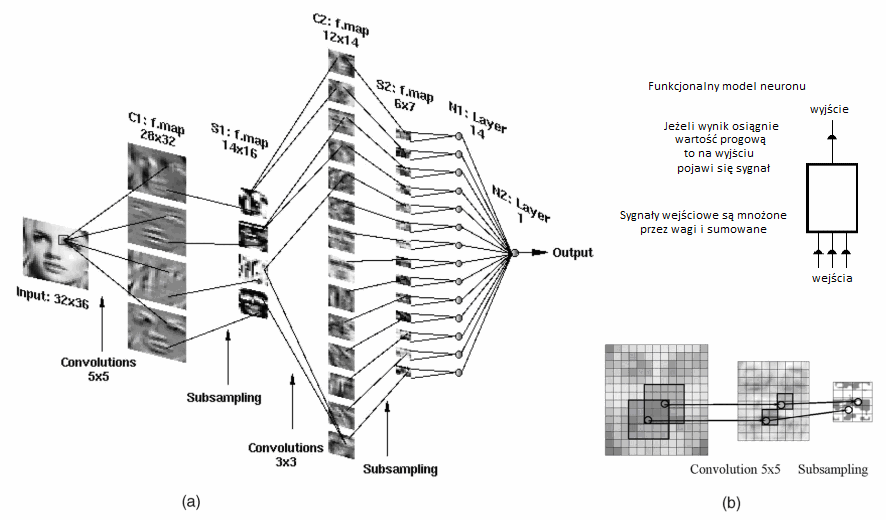
\includegraphics[scale=0.65]{cnn.png}
\vspace*{1cm}

\noindent 
Zalety:
\begin{itemize}
\item  Bardzo dobre rozpoznawanie wzorców
\item  Praca z zaszumianymi i niepełnymi danymi
\item  Możliwość pracy równoległa z wielu wejść
\item  Rozwiązanie problemu bez jego dogłębnej analizy
\item  Duża tolerancja na błędy
\end{itemize}

\noindent 
Wady:
\begin{itemize}
\item  Długi czas uczenia 
\item  Sukces uczenia nie jest gwarantowany 
\item  Problemy z wyborem danych do treningu sieci 
\end{itemize}

\subsection{Model aktywnego kształtu}
Tim Cootes i Chris Taylor w roku 1995 opracowali metodę modelu aktywnego kształtu (Active Shape Model)\cite{SMIA001}. Jest to model statyczny, w którym jego kształt poprzez dozwolone deformacje próbuje się automatycznie dopasowywać do obiektu znajdującego się na obrazie. Określa się wzorzec obiektu jako model rozkładu punktów (Point Distribution Model), czyli zbiór etykietowanych punktów określających poszukiwany kształt. Następnie przeprowadzany jest proces uczenia w którym zbiera się informacje o różnych modyfikacjach wzorca. W tym celu przeważnie na kolejne zdjęcia testowe twarzy nanosi są ręcznie punkty charakterystyczne. Otrzymane wektory punktów poddaje się procesowi normalizacji (taki model będzie można dowolnie przeskalowywać, zachowana jest jedynie informacja o kształcie). Na koniec należy obliczyć kształt średni, odchylenie od średniej dla każdego elementu zbioru uczącego oraz obliczyć wektory własne odpowiedniej macierzy kowariancji. Konstruuje się model utworzony z średniego kształtu i sumy ważonej najbardziej charakterystycznych deformacji. Algorytm pozwala na deformację kształtu średniego tylko w ograniczonym zakresie.\\
\\
\noindent
Lista kroków algorytmu wyszukiwania obiektu:
\begin{itemize}
\item Badane jest sąsiedztwo każdego punktu charakterystycznego w poszukiwaniu odpowiedniej deformacji
\item Obliczane są optymalne parametry przesunięcia, obrotu, skali tak aby umieścić niezdeformowany model jak najbliżej rzeczywistego kształtu
\item Uważając na dopuszczalny zakres zmian uaktualnia się parametry modelu dopasowując go jak najdokładniej do obrazu
\end{itemize}

Przesunięcie punktów charakterystycznych określa się na podstawie odnalezionych krawędzi znajdujących się na linii prostopadłej do brzegu modelu. Dysponując informacją o poziomach jasności wokół punktów modelu można też próbować odnajdywać miejsca w sąsiedztwie dla którego profil jasności najbardziej przypomina ten z modelu. \\

\vspace*{1cm}
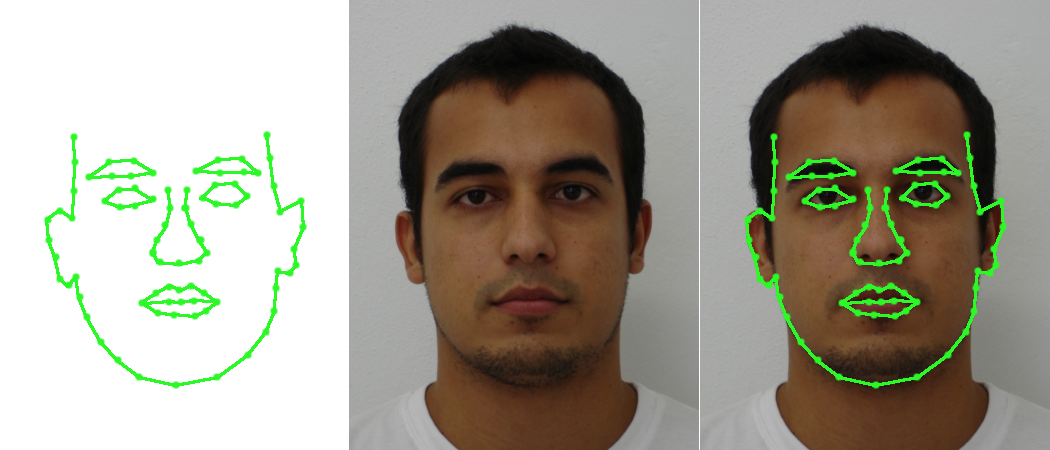
\includegraphics[scale=0.40]{active_shape.png}
\vspace*{1cm}

\noindent 
Zalety:
\begin{itemize}
\item Duża elastyczność - model potrafi dopasować się do różnych kształtów
\item Uniwersalny - kształt określany jest w drodze uczenia
\item Pomocny przy klasyfikowaniu i identyfikowaniu twarzy
\end{itemize}

\noindent 
Wady:
\begin{itemize}
\item  Czasochłonne i trudne uczenie modelu 
\item  Mało odporny na zmieniające się warunki oświetlenia, zróżnicowanego tła, bardziej realistycznych warunków
\item  Słabe wyniki dla osób z długimi ciemnymi włosami
\end{itemize}

\section{Porównanie}
Najstarszą z opracowywanych przez nas metod jest metoda geometryczna. Doczekała się licznych modyfikacji i dała ona początek oraz inspirację do wymyślania kolejnych. W ciągu kilkunastu lat powstało wiele coraz to lepszych rozwiązań. Pomimo ciekawego pomysłu i dobrych założeń metoda aktywnego kształtu okazała się mało użyteczna w normalnych warunkach. Natomiast znacznie bardziej obiecujące rezultaty można otrzymać stosując sieci neuronowe i podejście statystyczne.

\section{Podsumowanie}

Spośród omawianych przez nas metod każda ma zalety, ale też pewne słabości związane głównie ze zróżnicowanymi warunkami pozalaboratoryjnymi. W teorii osiąga się skuteczność na poziomie ponad 90\%. Życie jednak w praktyce weryfikuje przechwałki naukowców. Na przykład systemy automatycznego rozpoznawania przestępców w wielu krajach, które podjęły się pilotażowego ich wprowadzenia nie przyniosły wymiernych efektów \cite{SMIA002}. Mimo wszystko odnotowuje się kilkunasto do kilkudziesięcio procentową poprawę efektywności stosowanych metod z roku na rok. Problem pozostaje otwarty i coraz więcej ośrodków naukowych oraz wielkich korporacji prowadzi badania w tym kierunku. Organizowanych jest też wiele prestiżowych konkursów takich jak Face Recognition Grand Challenge \cite{FRGC001}.

\section{Bibliografia}

\bibliographystyle{plain}
\bibliography{bibliography}

\end{document}
